%!TEX root = thinkcs.tex

\section*{Analysis of Student Errors}

In the summer of 2013 we received a SIGCSE special projects grant to make several enhancements to our interactive textbooks, this included many projects:

\begin{itemize}
	\item A responsive design so the books were easy to read on tablets and phones as well as desktop computers.
	\item Adding answers to the odd numbered homework exercises
	\item Adding discussion areas for homework exercises
	\item Improving the error messages displayed to the students from activecode examples and exercises
\end{itemize}

One question we were particularly interested in exploring in the data set, was the impact of all of these changes to the exercises.  In particular we were intrigued by assertion in \ref{errors} that better error messages don't help students very much.  In our case, we had a lot of control over how error messages were displayed, and we had a year of data where error messages were simply displayed to students in an alert box, and a full year of data where we displayed error messages as shown in Figure~\ref{fig:newmess}.

\begin{figure}[htbp]
	\centering
		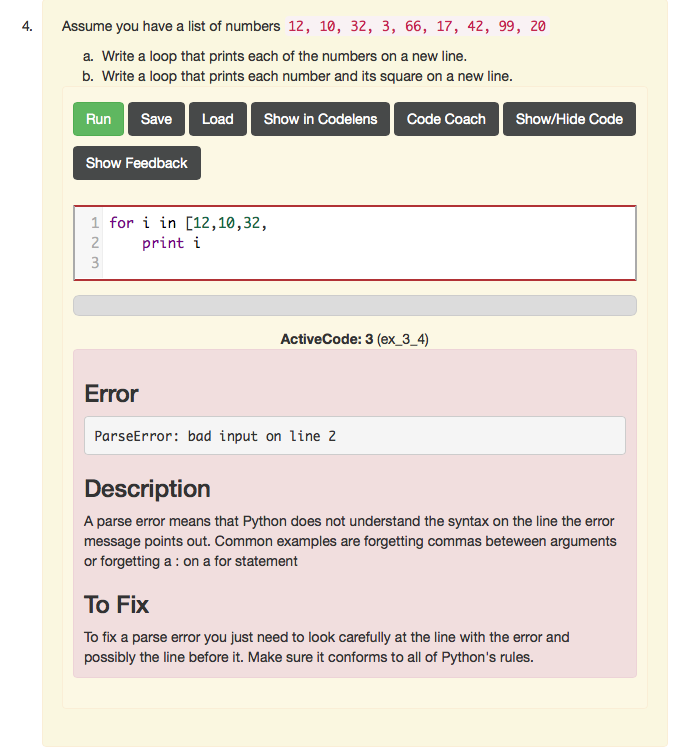
\includegraphics[scale=0.5]{emessage.png}
	\caption{A new style error message}
	\label{fig:newmess}
\end{figure}

As a Python instructor there are many interesting aspects of the exercises to compare from year one to year two.  

\begin{itemize}
	\item How ``efficient'' are students when they do their work?  How many attempts do they make to solve a particular problem?
	\item How often do they simply give up without solving the problem?
	\item What are the most common errors that students encounter?
	\item When students encounter an error how long does it take them to fix that particular error type?
	\item Are certain errors more problematic for students to fix than others?
\end{itemize}

To answer the first question we looked at the total number of times each student attempted the various end of the chapter programming exercises.  We only compared the even numbered questions since we had added the answers to the odd numbered questions in year two.  What we found was that overall from year one to year two the average number of attempts declined by 7.  Figure~\ref{fig:attempts} illustrates the difference on a per question basis.  You can see that nearly all of the questions had fewer attempts in the second year than the first.

\begin{figure}[htbp]
	\centering
		\includegraphics[scale=1]{errDiffs.png}
	\caption{caption}
	\label{fig:attempts}
\end{figure}



